\input{notes.tex}


\iftoggle{dualscreen}{\setbeameroption{show notes on second screen=right}}{}
\begin{document}
\section{Lecture 2}
\subsection{Introduction}

\slide[Recall:]{
Operator form of a DE:
\[\op{y(t)}  = f(t) \]
\vfill
For the next few weeks, we will focus on first order DEs\vfill
\[y\p = f(t,y).\]\vfill
We start with the two simple cases\vfill
\[ y\p = f(t) \quad \text{and} \quad y\p=f(y)\]
}

\subsection{Integrals as solutions}

\slide[Integrals as solutions]{\vspace{-1.25em}
\[ y\p = f(t) \quad \text{and} \quad y\p=f(y)\]
Strategy: \enum{\item Move everything that depends on $y$ to one side of the equal sign.\item Move everything that depends on $t$ to the other side. \item Integrate and isolate $y$.}\vfill
\ex{$y\p=\cos(t)$}
\student{\algn{\dd{y}{t} &= \cos(t) \\ \intop \text{d}y &= \intop \cos(t) \text{d}t \\ y(t) &=\sin(t) + C   \qquad \text{(General Solution)}}  }
}

\slide[Incorporating Initial Conditions]{
\ex{$y\p  = e^{-2t}$, with $y(0)=1$}
\student{\algn{ \dd{y}{t} &= e^{-2t} \\ 
 \intop \text{d}y &= \intop e^{-2t} \text{d}t  \\ 
y(t)  &= -\frac12 e^{-2t} + C   \qquad \text{(General Solution)} \intertext{impose the initial condition}
y(0)&= 1 = -\frac12 + C  \qquad \Rightarrow  \qquad C=1 +\frac12\\
\\ y(t)&=\frac32 - \frac12e^{-2t}   \qquad \text{(Particular Solution)}
}}
}


\slide{
\ex{$y\p = e^{2y}$, with y(1)=0}\student{
\algn{
 \dd{y}{t} &= e^{2y}
&\intop e^{-2y}\text{dy}  = \intop \text{d}t\\
-\frac12e^{-2y} & = t + C\\
e^{-2y} &= -2t-2C\\
y(t) &= -\frac12 \ln(-2t-2C) \intertext{impose the initial condition}
y(1) &= 0 = -\frac12 \ln(-2-2C) & \Rightarrow -2-2C = 1\\
&&C=-\frac32\\
y(t)&=-\frac12 \ln(-2t+3)
}
}
}
%\xcoord{2}{1}
\slide{
\ex{$y\p = e^{2y}$, with y(1)=0 \hspace{1em} $\Rightarrow$  \hspace{1em}  $y(t)=-\frac12 \ln(-2t+3)$}

\centering \vfill Solution blows-up in finite time!\vfill
\tikzplot[
\xcoord{4}{2}
\xcoord{2}{1}
\xcoord{-4}{-2}
\xcoord{-2}{-1}
\ycoord{1}{1}
\ycoord{2}{2}
\ycoord{-1}{-1}
]{5}{5}{1.5}{3}{t}{y(t)}{
\draw[domain=-2.5:1.5, thick, black, samples=500] plot ({2*\x},{-0.5*ln(-2*\x+3)});
}
\vfill
Domain of definition: \student{$t\in \left(-\infty,\frac32\right] $\vfill
Outside this domain, the solution does not exist.}
}

\slide[Separable Equations]{\vspace{-.5em}
Suppose you are given \[\frac{dy}{dx}=f(x)g(y)\] where the functions $f$ and $g$ are known. Proceeding as before...
\vfill
\student{\algn{
\frac{\text{d}y} {g(y)} &=f(t) dt\\
\int \frac{dy}{g(y)} &=\int f(t) dt\\
\Gamma(y) &=F(t) + C\\\\
y(t) &= \Gamma^{-1} \paren{F(t) + C}
}\vfill
Works as long as $1/g(y)$ and $f(t)$ are integrable functions.
}

}

\slide[]{\ex{$y'=-ty, \quad y(0)=5$}
%Can combine +- in exponent
}

\slide[]{\ex{ $\displaystyle \frac{dy}{dx}=\frac{x^2}{y}, \quad y(0)=1$}
%Have to choose +for square root. Solution only defined on interval
}


\slide[]{\ex{$y'=y^2 \quad y(0)=1$}
%Simple example of finite blowup
}

\slide[]{\ex{  $\frac{dy}{dt}=\sqrt{y}, \quad y(0)=0$	}


}

\slide[]{\ex{$y'=-xy, \quad y(0)=5$}
%Can combine +- in exponent
}


\begin{comment}
\subsection{ Graphical intuition and the direction field}

\slide[Graphical intuition, whats does $y\p = f(y,t)$ mean?]{\vspace{-.5em}
\twomini[.75]{.4}{.59}{
\tikzplot{1}{3.25}{1}{3.5}{t}{y(t)}{
\draw[thick, black] (0,3) .. controls (0,1) and (1,3) .. (3.5,-1);
\def\x0{1.6}
\def\y0{1.28}
\def\dx{.6}
\def\slope{-.77}
\def\spacer{.25}
\draw[ultra thick,->] (\x0-\dx,\y0-\dx*\slope) -- (\x0+\dx,\y0+\dx*\slope);
\node[vertex] at (\x0, \y0) {};
\draw[thick,|-|] (\x0-\dx,\y0+\dx*\slope-\spacer) -- (\x0+\dx,\y0+\dx*\slope-\spacer) node[midway, below]{$\Delta t$};
\draw[thick,|-|] (\x0-\dx-\spacer,\y0-\dx*\slope) -- (\x0-\dx-\spacer,\y0+\dx*\slope) node[midway, left]{$\Delta y$};
}


}
{

\[ \dd{y}{t} = f(y,t) \]

\student{
\vspace{.5em}
\algn{f(y,t) &= \text{slope of y(t) in the $(t,y)$-plane.}\\
&=\frac{\Delta y}{\Delta t}}
So, \[y(t+\Delta t) \approx y(t)+ \Delta t \cdot  f(y(t),t)\]


}
}
\student{\uline{Direction Field:} \enum{\item Draw the slope, $f(y,t)$, as an arrow for every point in the $(t,y)$-plane.
\item Connect the arrows to get qualitative (approximate) solutions.} }
}

\presentonly{
\slide[Example: $y\p=2-y$]{
\twomini{.4}{.6}{

\resizebox{5.25cm}{7cm}{
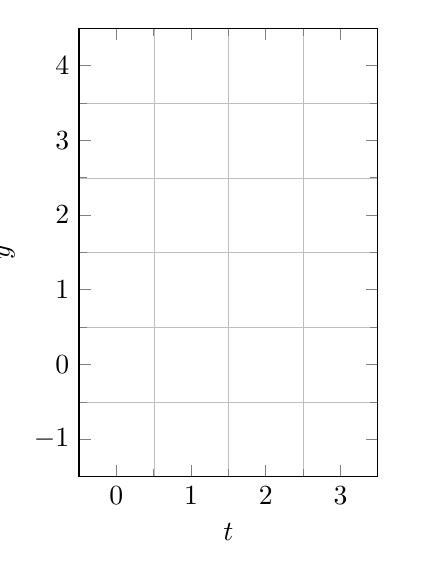
\begin{tikzpicture}\hspace{-.5cm}
\begin{axis}[
    xmin = -0.5, xmax = 3.5,
    ymin = -1.5, ymax = 4.5,
    zmin = 0, zmax = 1,
    grid=minor,
    grid style={line width=.1pt},
    major grid style={line width=.2pt},
    minor tick num=1,
    xtick = {0,1,2,3},
    ytick = {-1,0,1,2,3,4},
    axis equal image,
    view = {0}{90},
    xlabel={$t$},
    ylabel={$y$},
]



%    \addplot3[
%        quiver = {
%            u = {1/sqrt(1+(2-y)^2)},
%            v = {(2-y)/sqrt(1+(2-y)^2)},
%            scale arrows = 0.35,
%                every arrow/.append style={%
%                    line width=.1+\pgfplotspointmetatransformed/4000,
%                    -{Latex[length=0pt 5,width=0pt 3]}
%                }
%        },
%        -stealth,
%        domain = 0:3,
%        domain y = -1:4,
%        samples=16
%    ] {0};
%
\end{axis}

\end{tikzpicture}
}
}{
\enum{\item What type of solutions are possible? \student{\subitem{Monotonically increasing/decreasing}}\vspace{2em}
 \item What is $y(t)$ as $t\rightarrow\infty$?  \student{\subitem{Unique possibility: $y(t)\rightarrow2$ \item  $y=2$ is a stable steady state. }}\vspace{2em}
 \item What is the influence of the initial condition? \student{\subitem{If $y(0)>2$ decreasing solution. \item If $y(0)<2$ increasing solution.  \item If $y(0)=2$ constant solution. }}}
}

}
}

\fullonly{

\slide[Example: $y\p=2-y$]{
\twomini{.4}{.6}{

\resizebox{5.25cm}{7cm}{
\begin{tikzpicture}\hspace{-.5cm}
\begin{axis}[
    xmin = -0.5, xmax = 3.5,
    ymin = -1.5, ymax = 4.5,
    zmin = 0, zmax = 1,
    grid style={line width=.1pt},
    major grid style={line width=.2pt},
    xtick = {0,1,2,3},
    ytick = {-1,0,1,2,3,4},
    axis equal image,
    view = {0}{90},
    xlabel={$t$},
    ylabel={$y$},
]



    \addplot3[
        quiver = {
            u = {1/sqrt(1+(2-y)^2)},
            v = {(2-y)/sqrt(1+(2-y)^2)},
            scale arrows = 0.35,
                every arrow/.append style={%
                    line width=.1+\pgfplotspointmetatransformed/4000,
                    -{Latex[length=0pt 5,width=0pt 3]}
                }
        },
        -stealth,
        domain = -.5:3.5,
        domain y = -1.5:4.5,
        samples=16
    ] {0};

\end{axis}

\end{tikzpicture}
}
}{
\enum{\item What type of solutions are possible? \student{\subitem{Monotonically increasing/decreasing}}\vspace{2em}
 \item What is $y(t)$ as $t\rightarrow\infty$?  \student{\subitem{Unique possibility: $y(t)\rightarrow2$ \item  $y=2$ is a stable steady state. }}\vspace{2em}
 \item What is the influence of the initial condition? \student{\subitem{If $y(0)>2$ decreasing solution. \item If $y(0)<2$ increasing solution.  \item If $y(0)=2$ constant solution. }}}
}

}

}

\slide[Doesn’t the function $f(y,t)$ tell us everything?]{
More or less, it gives us all the qualitative properties of solutions.
\student{\itmz{\item Monotonic vs. Transiently Oscillatory vs. Periodic Solutions \item Steady states and their stability \item Influence of initial conditions}}
\vfill
So why bother integrating/solving DEs?
\student{\itmz{\item To get quantitative information. \item Impossible to graph direction fields for many systems of ODEs \item Drawing $f(y,t)$ is tedious when there is $t$-dependence.}}
}
%

\slide[Example: $y\p=y^2-t$]{
%
\vfill\resizebox{12cm}{7cm}{
\begin{tikzpicture}
\begin{axis}[
    xmin = 0, xmax = 7,
    ymin = -2, ymax = 3,
    zmin = 0, zmax = 1,
    axis equal image,
    view = {0}{90},
    xlabel={$t$},
    ylabel={$y$},
]
    \addplot3[
        quiver = {
            u = {1/sqrt(1+(y^2-x)^2)},
            v = {(y^2-x)/sqrt(1+(y^2-x)^2)},
            scale arrows = 0.25,
                every arrow/.append style={%
                    line width=.1+\pgfplotspointmetatransformed/4000,
                    -{Latex[length=0pt 5,width=0pt 3]}
                }
        },
        -stealth,
        domain = 0:7,
        domain y = -2:3,
        samples=24
    ] {0};
\end{axis}
\end{tikzpicture}}
\vfill

}

\slide[Summary]{
\enum{\item What are DEs?
\student{\subitem{Equations involving unknown function(s) and function derivatives. \item Specify rates of change of certain quantities. \item Useful for modelling many natural phenomena.}}\vfill
\item Terminology \student{\subitem{ODEs (\& PDEs). 
\item Order of DEs, systems of DEs, solutions to DEs, steady states.}}\vfill
\item Graphical Solutions (via Direction Fields)\student{ \subitem{ Intuitive way of thinking about DEs \item Provide qualitative information}}
}

}
\end{comment}
\end{document}